\documentclass[class=report, crop=false, 12pt,a4paper]{standalone}
\usepackage{enumitem}
\usepackage{multicol}
\usepackage{etoolbox}
\AtBeginEnvironment{quote}{\singlespacing\small}
\usepackage{setspace}
\onehalfspacing
\usepackage{graphicx}
\usepackage{float}
\usepackage{amsmath}
\usepackage{amssymb}
\usepackage{mathtools}
\usepackage{siunitx}
\sisetup{detect-all}
\begin{document}
\section{Momentum equation}
\begin{equation}
  \sum F_{sys} = \frac{\partial}{\partial t} \int_{CV} \underline{V} \rho d \forall + \int_{CS} \rho \underline{V} (\underline{V} \cdot \underline{n}) dA
\end{equation}
\subsection{Vane example:}
A horizontal jet of water exits a nozzle with a uniform speed of $V_1 = 3.048$ \si{\meter\per\second}, strikes a vane and is turned through an angle $\theta$. Determine the anchoring force needed to hold the vane stationary if gravity and visocus effects are negligible. 
\begin{figure}[h]
  \centering
  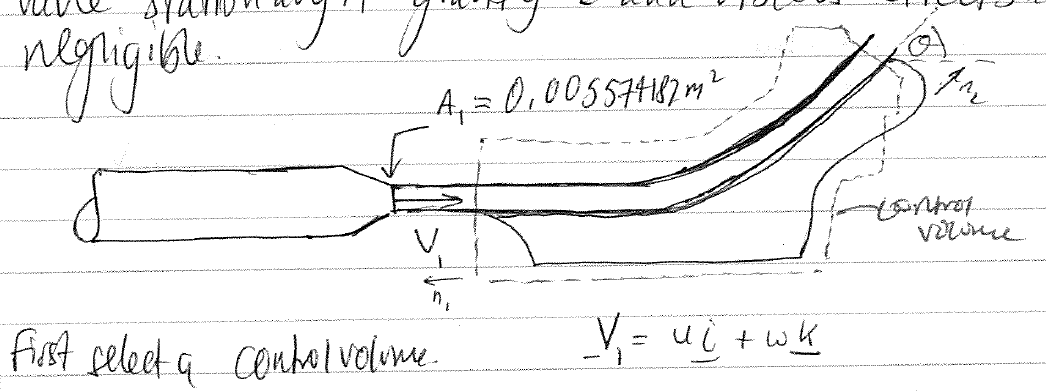
\includegraphics[width = 0.9\textwidth]{../img/Vanexample}
  \caption{Water flow through vane system.}
\end{figure}
The only portions of the control surfrace across which fluid flows are section 1 (the entrance) and section 2 (the exit). Hence, the momentum equation becomes in the x and z components.
\begin{align}
  \sum F_x &= \int_{inlet} u \rho (\underline{v} \cdot \underline{n}) dA + \int_{outlet} u \rho (\underline{V} \cdot \hat{n}) dA\\
  \sum F_x &= u_1 \rho (-V_1) A_1 + u_2 \rho (V_2) A_2\\
  \sum F_x &= u_2 \rho A_2 V_2 - i_1 \rho A_1 V_1
\end{align}
In the z direction:
\begin{align}
  \sum F_z &= \int_{inlet} w \rho (\underline{V}\cdot \hat{n}) dA + \int_{outlet} w \rho (\underline{V} \cdot {n}) dA\\
  \sum F_z &= w_2 \rho A_2 V_2 - w_1 \rho A_1 V_1
\end{align}
We know that at inlet $V_1$ there is no vertical component, hence $w_1 = 0$ and $u_1 = V_1$. At the outlet:
\begin{figure}
  \centering
  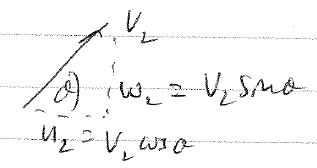
\includegraphics[width = 0.7\textwidth]{../img/Vanexample2}
  \caption{Velocity components at outlet.}
\end{figure}
Also lets find $V_1$ and $V_2$. From Bernoulli's equation (neglecting g, assuming incompressible and that $P_1 = P_2 = P_{atm}$), $V_1 = V_2$.
\begin{align}
  \therefore \sum F_z &= V_2 \sin{\theta} \rho A_2 V_2 = V_1^2 A_2 \sin{\theta} \rho \\
  \sum F_x &= V_2 \cos{\theta} \rho A_2 V_2 - V_1 \rho A_1 V_1\\
  \sum F_x &= V_1^2 A_2 \cos{\theta} \rho - V_1^2 \rho A_1 \\
  \sum F_x &= V_1^2 (A_2 \cos{\theta} \rho - \rho A_1)
\end{align}
\begin{figure}
  \centering
  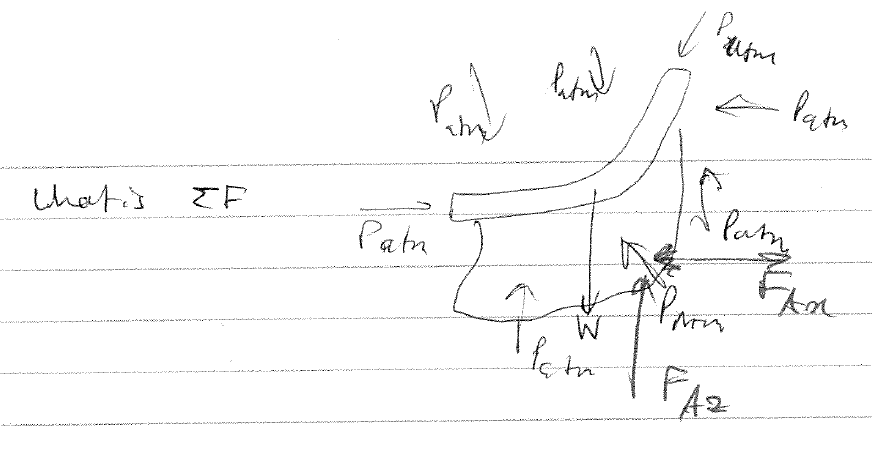
\includegraphics[width = 0.8\textwidth]{../img/Vanexample3}
  \caption{Forces acting on system.}
\end{figure}
Neglect $w$ and the net force due to $P_{atm} = 0$
\begin{align}
  \therefore \sum F_x &= F_{Ax}\\
  \sum F_z &= F_{Az}\\
  F_{Ax} &= V_1^2 A_2 \sin{\theta} \rho\\
  F_{Az} &= V_1^2 (A_z \cos{\theta} \rho - \rho A_1)
\end{align}
Also remember that,
\begin{align}
  \dot{m}_1 &= \dot{m}_2\\
  V_1 A_1 &= V_2 A_2 \textrm{ (incompressibility)}\\
  V_1 = V_2 &\therefore A_1 = A_2\\
  \therefore F_{Ax} &= V_1^2 A_1 \sin{\theta} \rho \\
  F_{Az} = \rho V_1^2 (A_1 \cos{\theta} - A_1) &= \rho V_1^2 A_1 (\cos{\theta} - 1)
\end{align}
Plug in data to find $F_{Ax}$ and $F_{Az}$.
\section{Calculating the thrust produced by \\ a propeller}
We want to know the thrust applied by the propeller and the total work done. We will assume that there is are no losses due to friction or viscosity. There are three stages to this: 
\begin{enumerate}[noitemsep]
  \item Use Bernoulli's equation to derive an expression for thrust.
  \item Use the momentum equation to derive an independent equation for the thrust.
  \item Combine these two equations to solve for the speed of the propeller.
\end{enumerate}
\begin{figure}
  \centering
  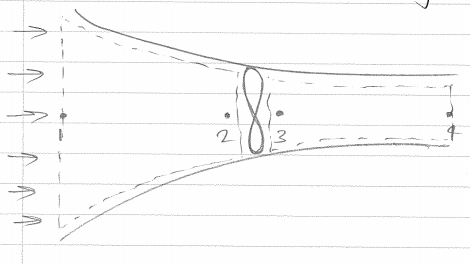
\includegraphics[width = 0.7\textwidth]{../img/PropDiagram}
  \caption{Diagram of a propeller with the flow going from left to right.}
\end{figure}
\begin{enumerate}[noitemsep]
  \item Create a control volume. 
  \item Apply Bernoulli's equation between points 1 and 2:
    \begin{equation}
      P_1 + \frac{1}{2} \rho V_1^2 = P_2 + \frac{1}{2} \rho V_1^2
    \end{equation}
  \item Apply Bernoulli's equation between points 3 and 4:
    \begin{equation}
      P_3 + \frac{1}{2} \rho V_3^2 = P_4 + \frac{1}{2} \rho V_4^2
    \end{equation}
  \item $P_1 = P_4 = P_{atm}$, so rearrange these two equations and equate:
    \begin{gather}
      P_1 = P_2 + \frac{1}{2}\rho (V_2^2 - V_1^2)\\
      P_4 = P_3 + \frac{1}{2}\rho (V_3^2 - V_4^2)\\
      P_2 + \frac{1}{2}\rho (V_2^2 - V_1^2) = P_3 + \frac{1}{2}\rho (V_3^2 - V_4^2)
    \end{gather}
  \item We can now say that the velocity change across the propeller is small such that $V_2 \approx V_3$, so we can write.
    \begin{gather}
      \Delta P = P_3 - P_2 = \frac{1}{2} \rho [ V_4^2 - V_1^2] = \frac{1}{2} \rho [V_4^2 - V_1^2]\\
      \therefore \Delta P = \frac{1}{2} \rho (V_4^2 - V_1^2)
    \end{gather}
  \item The thrust $F$ provided by the pressure must be equal to the pressure difference multiplied by the area of the propellers. 
    \begin{gather}
      \therefore F = \Delta P \times A\\
      F = \frac{1}{2} \rho A (V_4^2 - V_1^2) \label{thrustprop}
    \end{gather}
  \item Now we use the momentum equation to derive another expression for the force. Force exerted on this central volume is given by the momentum equation. 
    \begin{equation}
      \sum F = \frac{\partial}{\partial t} \int_{CV} \rho \underline{V} d \forall + \int_{CS} \rho \underline{V} (\underline{V} \cdot \underline{\hat{n}}) dA
    \end{equation}
    Assume steady flow, hence $\frac{\partial}{\partial t} \int_{CV} \rho \underline{V} d \forall =0$
      \begin{gather}
        \sum F_x = \int_{CS} \rho \underline{V} (\underline{V} \cdot \underline{\hat{n}}) dA = \int_{inlet} \rho V_1 (-V_1) dA + \int_{output} \rho V_4 (V_4) dA\\
        = -\dot{m}_1 V_1 + \dot{m}_4 V_4
      \end{gather}
    Assume steady flow, neglect gravity and viscous forces: $\dot{m}_1 = \dot{m}_4$
      \begin{equation}
        F = \dot{m}(V_4 - V_1)
      \end{equation}
  \item But at the propeller the mass flow rate equals:
    \begin{gather}
      \dot{m} = \rho A_P \times V_P = \rho A V_P
      \therefore F = \rho A V_P (V_4 - V_1) \label{thrustprop2}
    \end{gather}
  \item Equate equations (\ref{thrustprop}) and (\ref{thrustprop2})
    \begin{gather}
      F = V_P (V_4 - V_1) = \frac{1}{2}(V_4^2 - V_1^2)\\
      V_P = \frac{1}{2}\frac{(V_4 - V_1)(V_4 + V_1 )}{(V_4 - V_1)}\\
      V_P = \frac{1}{2}(V_4 + V_1 )
    \end{gather}
  \item Now using given data, you can work out $V_P$ and thus find the thrust and the work done.
\end{enumerate}
\subsection{Moving control volume}
Let us recap on the RTT:
\begin{equation}
  \frac{DB_{sys}}{Dt} = \frac{\partial}{\partial t} \int_{CV} \rho b d \forall + \int_{CS} \rho b (\underline{V}\cdot \underline{\hat{n}}) dA 
\end{equation}
For mass conservation:
\begin{equation}
  0 = \frac{\partial}{\partial t} \int_{CV} \rho d \forall + \int_{CS} \rho (\underline{V}\cdot \underline{\hat{n}}) dA 
\end{equation}
For momentum equation:
\begin{equation}
  \sum F_{sys} = \frac{\partial}{\partial t} \int_{CV} \rho \underline{V} d \forall + \int_{CS} \rho \underline{V} (\underline{V}\cdot \underline{\hat{n}}) dA 
\end{equation}
What if the control volume is moving around, in an inertial reference frame: not accelerating? Our $\underline{V} \cdot \underline{\hat{n}}$ terms pertains to the net mass flow out relative to that boundary.
\begin{figure}
  \centering
  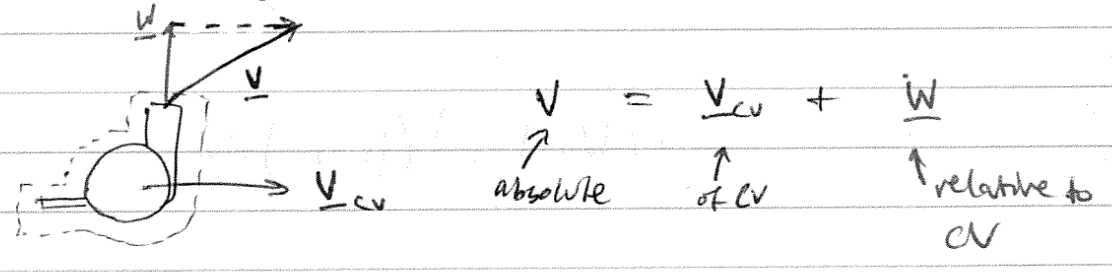
\includegraphics[width = \textwidth]{../img/RTTMovingControlVolume}
\end{figure}
\subsubsection{Conservation of mass}
\begin{align}
  \textrm{original} \rightarrow 0 &= \frac{\partial}{\partial t} \int_{CV} \rho d \forall + \int_{CS} \rho (\underline{V}\cdot \underline{\hat{n}}) dA \\
  \textrm{moving inertial} \rightarrow 0 &= \frac{\partial}{\partial t} \int_{CV} \rho d \forall + \int_{CS} \rho (\underline{W}\cdot \underline{\hat{n}}) dA
\end{align}
When in steady state, first term cancels,
\begin{equation}
  0 = \int_{CS} \rho (\underline{W}\cdot \underline{\hat{n}}) dA 
\end{equation}
Mass crosses boundary due to the relative velocity, not the absolute.
\subsubsection{Inertial moving object: conservation of momentum}
\begin{equation}
  \textrm{original} \rightarrow \sum F_{sys} = \frac{\partial}{\partial t} \int_{CV} \rho \underline{V} d \forall + \int_{CS} \rho \underline{V} (\underline{V}\cdot \underline{\hat{n}}) dA 
\end{equation}
Swap $\underline{V}$ for $\underline{W}$ in the second integral's bracket as the bracket relates to the mass flow out, relative to the boundary. 
\begin{equation}
  \sum F_{sys} = \frac{\partial}{\partial t} \int_{CV} \rho \underline{V} d \forall + \int_{CS} \rho \underline{V} (\underline{W}\cdot \underline{\hat{n}}) dA 
\end{equation}
Since
\begin{align}
  \underline{V} &= \underline{V}_{CV} + \underline{W}\\
  \frac{\partial}{\partial t} \int_{CV} \rho (\underline{V}_{CV} + \underline{W}) d \forall &= 0 \rightarrow \textrm{steady state}\\
  \sum F_{sys} &= \int_{CS} \rho (\underline{V}_{CV} + \underline{W}) (\underline{W}\cdot \underline{\hat{n}}) dA \\
  \sum F_{sys} &= \int_{CS} \rho \underline{W}(\underline{W}\cdot \underline{\hat{n}}) dA + \underline{V}_{CV} \int_{CS} \rho (\underline{W}\cdot \underline{\hat{n}}) dA
\end{align}
Second term is equal to zero due to steady state flow and mass conservation
\begin{equation}
  \sum F_{sys} = \int_{CS} \rho (\underline{W})(\underline{W}\cdot \underline{\hat{n}}) dA 
\end{equation}
Hence, steady state conservation of momentum for a moving object in an inertial reference frame is: 
\begin{equation}
  \sum F_{sys} = \int_{CS} \rho \underline{W} (\underline{W}\cdot \underline{\hat{n}}) dA
\end{equation}
\section{The energy equation}
Review:
\begin{equation}
  \frac{DB_{sys}}{dt} = \frac{\partial}{\partial t} \int_{CV} \rho b d \forall + \int_{CS} \rho b (\underline{V}\cdot \underline{\hat{n}}) dA
\end{equation}
Let $B=E \therefore b = \frac{E}{m} = e = u + ke + pe = u + \frac{V^2}{2} + gz$.
\begin{equation}
  \frac{DE_{sys}}{dt} = \frac{\partial}{\partial t} \int_{CV} \rho e d \forall + \int_{CS} \rho e (\underline{V}\cdot \underline{\hat{n}}) dA
\end{equation}
Also recall from first law of thermodynamics that, $\Delta E = \Delta KE + \Delta PE + \Delta U = \Delta Q + \Delta W$.
\begin{gather}
  \dot{E} = \dot{Q}_{in} - \dot{Q}_{out} + \dot{W}_{in} - \dot{W}_{out}\\
  \frac{DE_{sys}}{dt} = (\dot{Q}_{in} - \dot{Q}_{out}) + (\dot{W}_{in} - \dot{W}_{out})\\
  \frac{DE_{sys}}{dt} = \left( \sum \dot{Q}_{\textrm{net in}} + \sum \dot{W}_{\textrm{net in}} \right)_{sys} \label{energyeq1}
\end{gather}
For a control volume that is coincident with the system at an instant in time.
\begin{equation}
  \left( \sum \dot{Q}_{\textrm{net in}} + \sum \dot{W}_{\textrm{net in}} \right)_{sys} = \left( \sum \dot{Q}_{\textrm{net in}} + \sum \dot{W}_{\textrm{net in}} \right)_{\textrm{coincident control volume}}
\end{equation}
Hence,
\begin{equation}
  \frac{D}{Dt} \int_{sys} e \rho d \forall = \left( \sum \dot{Q}_{\textrm{net in}} + \sum \dot{W}_{\textrm{net in}} \right)_{\textrm{coincident control volume}} \label{energyeq2}
\end{equation}
Equation (\ref{energyeq1}) = Equation (\ref{energyeq2})
\begin{equation}
  \therefore \left[ \sum \dot{Q}_{\textrm{net in}} + \sum \dot{W}_{\textrm{net in}} \right]_{CV} = \frac{\partial}{\partial t} \int_{CV} e \rho d \forall + \int_{CS} e \rho (\underline{V} \cdot \underline{\hat{n}}) dA \label{energyeq3}
\end{equation}
\subsection{Different forms of work}
\subsubsection{Shaft work}
\begin{align}
  \dot{W}_{shaft} &= T_{shaft} \omega\\
  \dot{W}_{\textrm{shaft net in}} &= \sum \dot{W}_{shaft in} - \sum \do{W}_{\textrm{shaft out}}
\end{align}
\subsubsection{Flow work}
\begin{gather}
  \dot{W}_{\textrm{normal stress}} = \int_{CS} \sigma (\underline{V}\cdot \hat{n}) dA\\
  = - \int_{CS} P (\underline{V}\cdot \hat{n}) dA\\
  \textrm{where } \sigma \ (\textrm{local normal stress}) = - P \ (\textrm{fluid pressure})\\
  (\delta \dot{W}_{\textrm{normal stress}} = \delta F_{\textrm{normal stress}} \cdot V = \sigma \underline{\hat{n}} \delta A \cdot \underline{V} = -P\underline{V} \cdot \underline{\hat{n}} \delta A )
\end{gather}
Therefore, equation (\ref{energyeq3}) becomes,
\begin{gather}
  \dot{Q}_{\textrm{net in}} + \dot{W}_{\textrm{net in}} = \frac{\partial}{\partial t} \int_{CV} e \rho d \forall + \int_{CS} e \rho (\underline{V} \cdot \underline{\hat{n}}) dA\\
  \dot{Q}_{\textrm{net in}} + \dot{W}_{\textrm{shaft net in}} + \dot{W}_{\textrm{normal stress}} = \frac{\partial}{\partial t} \int_{CV} e \rho d \forall + \int_{CS} e \rho (\underline{V} \cdot \underline{\hat{n}}) dA\\
  \dot{Q}_{\textrm{net in}} + \dot{W}_{\textrm{shaft net in}} - \int_{CS} P (\underline{V}\cdot \hat{n}) dA = \frac{\partial}{\partial t} \int_{CV} e \rho d \forall + \int_{CS} e \rho (\underline{V} \cdot \underline{\hat{n}}) dA
\end{gather}
Rearranging gives,
\begin{gather}
  \dot{Q}_{\textrm{net in}} + \dot{W}_{\textrm{shaft net in}} = \int_{CS} P (\underline{V}\cdot \hat{n}) dA + \frac{\partial}{\partial t} \int_{CV} e \rho d \forall + \int_{CS} e \rho (\underline{V} \cdot \underline{\hat{n}}) dA
\end{gather}
Factorise $\rho (\underline{V}\cdot \underline{\hat{n}})$
\begin{gather}
  \dot{Q}_{\textrm{net in}} + \dot{W}_{\textrm{shaft net in}} = \frac{\partial}{\partial t} \int_{CV} e \rho d \forall + \int_{CS} \rho (\underline{V} \cdot \underline{\hat{n}})(e + \frac{P}{\rho}) dA\\
  \dot{Q}_{\textrm{net in}} + \dot{W}_{\textrm{shaft net in}} = \frac{\partial}{\partial t} \int_{CV} e \rho d \forall + \int_{CS} \rho (\underline{V} \cdot \underline{\hat{n}})(u + \frac{P}{\rho} + \frac{V^2}{2} + gz) dA
\end{gather}
\subsection{Application of the energy equation}
When steady, $\frac{\partial}{\partial t} \int_{CV} e \rho d \forall$ cancels out or when flow is steady in the mean (cyclical). Also, in the second term, the integrand can be non zero only where the fluid crosses the surface. If the properties are all assumed to be uniformly distributed then the integration becomes simple and gives:
\begin{gather}
  \int_{CS} (u + \frac{P}{\rho} + \frac{V^2}{2} + gz) \rho (\underline{V} \cdot \hat{n}) dA\\
  = \sum_{\textrm{flow out}} \dot{m} (u + \frac{P}{\rho} + \frac{V^2}{2} + gz) - \sum_{\textrm{flow in}} \dot{m} (u + \frac{P}{\rho} + \frac{V^2}{2} + gz)
\end{gather}
If only one stream is coming in and out:
\begin{equation}
  = \dot{m}_{out} (u + \frac{P}{\rho} + \frac{V^2}{2} + gz)_{out} - \dot{m}_{in} (u + \frac{P}{\rho} + \frac{V^2}{2} + gz)_{in}
\end{equation}
For steady flow, $\dot{m}_{in} = \dot{m}_{out} = \dot{m}$, therefore, the energy equation becomes:
\begin{multline}
  \dot{Q}_{\textrm{net in}} + \dot{W}_{\textrm{shaft net in}} = \\
  \dot{m} \left[ u_{out} - u_{in} + \left( \frac{P}{\rho} \right)_{out} - \left( \frac{P}{\rho} \right)_{in} + \frac{V_{out}^2 - V_{in}^2}{2} + g(z_{out} - z_{in}) \right]
\end{multline}
\subsection{Comparison of the energy equation and the \\ Bernoulli equation}
For an incompressible and steady flow which consists of no shaft work:
\begin{equation}
  \dot{Q}_{\textrm{net in}} = \dot{m} \left[ u_{out} - u_{in} + \frac{P_{out}}{\rho} - \frac{P_{in}}{\rho} + \frac{V_{out}^2 - V_{in}^2}{2} + g(z_{out} - z_{in}) \right]
\end{equation}
Divide by $\dot{m}$ and rearranging. $(\frac{Q_{\textrm{net in}}}{\dot{m}} = q_{\textrm{net in}})$.
\begin{equation}
  \frac{P_{out}}{\rho} + \frac{V_{out}^2}{2} + gz_{out} = \frac{P_{in}}{\rho} + \frac{V_{in}^2}{2} + gz_{in} - (u_{out} - u_{in} - q_{\textrm{net in}})
\end{equation}
Loss $= (u_{out} - u_{in} - q_{\textrm{net in}})$.
\begin{equation}
  \therefore \frac{P_{out}}{\rho} + \frac{V_{out}^2}{2} + gz_{out} = \frac{P_{in}}{\rho} + \frac{V_{in}^2}{2} + gz_{in} - \textrm{Loss}
\end{equation}
When the problem includes incompressible one-dimensional, steady in the mean flow, with friction and shaft work (e.g. in pumps, blowers, fans and turbines), then we need to include shaft work.
\begin{gather}
  \therefore \frac{P_{out}}{\rho} + \frac{V_{out}^2}{2} + gz_{out} = \frac{P_{in}}{\rho} + \frac{V_{in}^2}{2} + gz_{in} + w_{\textrm{shaft net in}} - \textrm{Loss}\\
  (w_{\textrm{shaft net in}} = \frac{\dot{W}_{\textrm{shaft net in}}}{\dot{m}})
\end{gather}
To calculate the efficiency, we calculate the ratio of work that produces a useful effect $(w_{\textrm{shaft net in}} - \textrm{Loss})$ to the amount of work delivered to the fan blades.
\begin{align}
  \eta &= \frac{w_{\textrm{shaft net in}} - \textrm{Loss}}{w_{\textrm{shaft net in}}}\\
  \textrm{where loss} &= (u_{out} - u_{in} - q_{\textrm{net in}})\\
  \eta &= \frac{w_{\textrm{shaft net in}} - (u_{out} - u_{in} - q_{\textrm{net in}})}{w_{\textrm{shaft net in}}}
\end{align}
\end{document}